\section{Einleitung} % (fold)
\label{sec:einleitung}

	
	$\alpha$-Teilchen geben in Materie Energie durch elastische St"o"se, aber auch Anregungs- und Dissoziationsproze"se ab. In diesem Versuch soll nun bestimmt werden, welche Reichweite die $\alpha$-Strahlung in Luft bei verschiedenen Luftdr"ucken besitzt.
	
\section{Theorie} % (fold)
\label{sec:theorie}

\subsection{$\alpha$-Strahlung} % (fold)
\label{sub:_alpha_strahlung}

$\alpha$-Strahlung ist eine der drei Strahlungen, welche beim radioaktiven Zerfall instabiler Atomkerne auftritt.
Dabei sinkt die Kernladungszahl des Atoms und ein Heliumkern, die $\alpha$-Strahlung, wird emittiert.

\subsection{Reichweite von $\alpha$-Strahlung} % (fold)
\label{sub:reichweite_von_alpha_strahlung}

Neben elastischen St"o"sen und Ionisationsprozessen k"onnen $\alpha$-Teilchen ihre Energie auch durch Anregung oder Dissoziaion von Molek"ulen verlieren. Der Energieverlust pro Strecke ist dabei von der Energie der Strahlung und der Dichte des durchlaufenden Materials ab.

F"ur hinreichend gro"se Energien l"asst sich dies durch die Bethe-Bloch-Gleichung beschreiben, da bei niedrigen Energien Lad
ungsaustauschproze"se vermehrt auftauchen:

\begin{equation}
	-\frac{\mathrm{d}E_\mathrm{\alpha}}{\mathrm{d}x} = \frac{z^2e^4}{4\pi \epsilon_\mathrm{0} m_\mathrm{e}} \frac{n Z}{v^2} \ln \left( \frac{2 m_\mathrm{e}v^2}{I} \right)
\end{equation}

dabei ist $z$ die Ladung und $v$ die Geschwindigkeit der $\alpha$-Strahlung. $Z$ ist die Ordnungszahl, $n$ die Teilchendichte und $I$ die Ionisierungsenergie des Targetgases.

Die Reichtweite $R$ l"asst sich nun schreiben als:

\begin{equation}
	R = \int_0^E_\mathrm{0} \frac{\mathrm{d}E_\mathrm{\alpha}}{- \frac{\mathrm{d}E_\mathrm{\alpha}}{\mathrm{d}x}}
\end{equation}

Bei $\alpha$-Strahlung in Luft mit Energien von $E_\mathrm{\alpha} <= \SI{2.5}{\mega\electronvolt}$ gilt:

\begin{equation}
	R_\mathrm{m} = 3.1 \cdot E_\mathrm{\alpha}^\frac{3}{2}
\end{equation}

In Gasen bei konstaner Temperatur und konstantem Volumen ist die Reichweite von $\alpha$-Teilchen proportional zum Druck $p$. Daher kann durch variieren des Drucks $p$ eine Absorptionsmessung gemacht werden. Es gilt f"ur einen festen Abstand $x_\mathrm{0}$ zwischen Detektor und $\alpha$-Strahler:

\begin{equation}
	x = x_\mathrm{0} \frac{p}{\SI{1013}{\milli\bar}}
\end{equation}

\subsection{Halbleiter-Sperrschichtz"ahler} % (fold)
\label{sub:halbleiter_sperrschichtz_ahler}


\begin{wrapfigure}{r}{7cm}
	\centering
	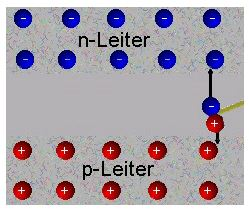
\includegraphics[width = 7cm]{img/pn.JPG}
	\caption{Schematische Darstellung eines Halbleitersperrschichtz"ahlers \cite{pn}.}
	\label{fig:pn}
\end{wrapfigure}

Zwischen einer p- und einer n-dotierten Halbleiterschicht bildet sich eine Ladungsfreie Zone aus. Durch das Anlegen einer Spannung in Sperrichtung wird diese vergr"o"sert.

Dringt nun ein ionisierendes Teilchen in diese Zone ein, werden Paare von Elektronen und L"ochern erzeugt.

L"ocher werden durch das starke elektrische Feld in dieser Zone in die p-dotierte, Elektronen in die n-dotierte Schicht gezogen.

Diese f"uhren zu einem Stromimpuls. Je gr"o"ser die Energie der einfliegenden Teilchen ist, desto mehr Elektornen-Loch-Paare werden erz"augt. Somit ist das gemessene Signal proprtional zur Energie des Teilchens.

\subsection{Diskreminatorschwelle} % (fold)
\label{sub:diskreminatorschwelle}

Die Diskreminatorschwelle beurteilt einen Me"swert. Dieser wird mit einem Schwellenwert verglichen und wenn dieser dar"uber liegt wird dieser gemessen. Ansonsten wird dieser verworfen.